
% \section{Vorticity and Potential Vorticity}
\begin{frame}{Was ist Vortizität?}
	\begin{columns}
		\column{0.99\textwidth}
		\begin{itemize}
			\item \textbf{Vortizität} beschreibt die lokale Rotation in einer Strömung.
			\item Definiert als das \textbf{Rotationsfeld} des Geschwindigkeitsfeldes:
			      \[
				      \vec{\zeta} = \nabla \times \vec{u}
			      \]
			\item Für eine zweidimensionale Strömung \( \vec{u} = (u(x,y), v(x,y)) \) ist nur die \(z\)-Komponente relevant:
			      \[
				      \zeta = \dfrac{\partial v}{\partial x} - \frac{\partial u}{\partial y}
			      \]
			\item \(\zeta > 0\): Zyklonale Rotation (gegen den Uhrzeigersinn)
			\item \(\zeta < 0\): Antizyklonale Rotation (im Uhrzeigersinn)
		\end{itemize}

		\column{0.4\textwidth}
		\vspace{2cm}  % Optional für vertikale Ausrichtung
	\end{columns}
\end{frame}


\begin{frame}{Zero Vorticity (Uniform Flow)}
	\begin{columns}
		\column{0.5\textwidth}
		\begin{itemize}
			\item \( \vec{u} = (2, 0) \)
			\item Uniform horizontal flow
			\item No shear or curvature
			\item \( \zeta = \dfrac{\partial v}{\partial x} - \dfrac{\partial u}{\partial y} = 0-0= 0 \)
		\end{itemize}

		\column{0.5\textwidth}
		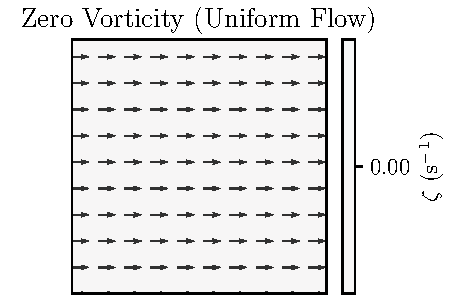
\includegraphics[width=\linewidth]{../images/vorticity_plot0.pdf}
	\end{columns}
\end{frame}

\begin{frame}{Shear Vorticity}
	\begin{columns}
		\column{0.5\textwidth}
		\begin{itemize}
			\item \( \vec{u} = (y, 0) \)
			\item Horizontal shear: \( \dfrac{\partial u}{\partial y} = 1 \)
			\item \( \zeta = \dfrac{\partial v}{\partial x} - \dfrac{\partial u}{\partial y} = 0-1= -1 \)
		\end{itemize}

		\column{0.5\textwidth}
		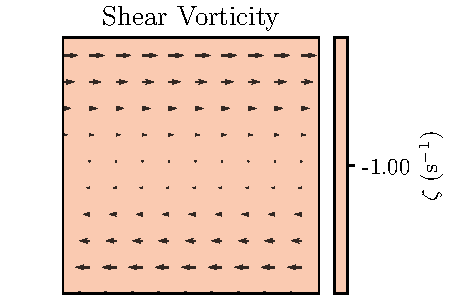
\includegraphics[width=\linewidth]{../images/vorticity_plot1.pdf}
	\end{columns}
\end{frame}

\begin{frame}{Nonlinear Shear Vorticity}
	\begin{columns}
		\column{0.5\textwidth}
		\begin{itemize}
			\item \( \vec{u} = (y^2, 0) \)
			\item Antisymmetric vorticity field
			\item Stronger at larger \( |y| \)
			\item \( \zeta = \dfrac{\partial v}{\partial x} - \dfrac{\partial u}{\partial y} = 0-2y = -2y \)

		\end{itemize}

		\column{0.5\textwidth}
		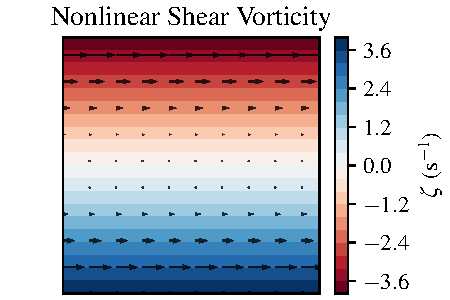
\includegraphics[width=\linewidth]{../images/vorticity_plot2.pdf}
	\end{columns}
\end{frame}

\begin{frame}{Positive Vorticity (Cyclonic)}
	\begin{columns}
		\column{0.5\textwidth}
		\begin{itemize}
			\item \( \vec{u} = (-y, x) \)
			\item Pure rotation, counter-clockwise
			\item \( \zeta =  \dfrac{\partial v}{\partial x} - \dfrac{\partial u}{\partial y} = 1-(-1)=2 \)
		\end{itemize}

		\column{0.5\textwidth}
		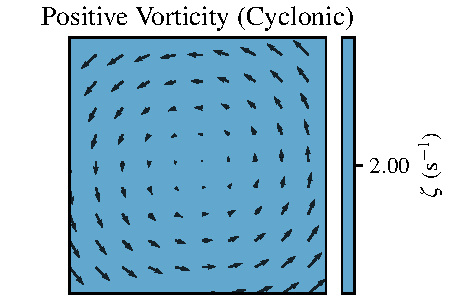
\includegraphics[width=\linewidth]{../images/vorticity_plot3.pdf}
	\end{columns}
\end{frame}

\begin{frame}{Negative Vorticity (Anticyclonic)}
	\begin{columns}
		\column{0.5\textwidth}
		\begin{itemize}
			\item \( \vec{u} = (y, -x) \)
			\item Clockwise rotation
			\item \( \zeta = \dfrac{\partial v}{\partial x} - \dfrac{\partial u}{\partial y} = -1-1=-2 \)
		\end{itemize}

		\column{0.5\textwidth}
		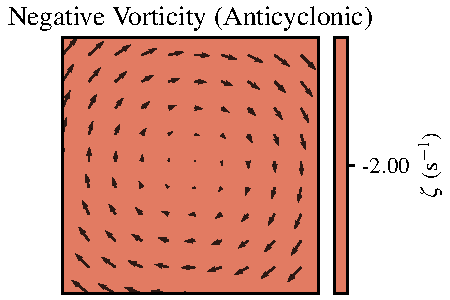
\includegraphics[width=\linewidth]{../images/vorticity_plot4.pdf}
	\end{columns}
\end{frame}

\begin{frame}{Absolute Vortizität}
	\begin{columns}
		\column{0.99\textwidth}
		\begin{itemize}
			\item In einem rotierenden Bezugssystem (wie der Erde) ergibt sich die \textbf{absolute Vortizität} zu:
			      \[
				      \eta = f + \zeta
			      \]
			\item \( \zeta \): relative Vortizität (durch Scherung und Krümmung der Strömung)
			\item \( f = 2\Omega \sin\phi \): Coriolis-Parameter, abhängig von der geografischen Breite
		\end{itemize}

		\column{0.4\textwidth}
		\vspace{2cm}
	\end{columns}
\end{frame}


\begin{frame}{Konservierung der potentiellen Vortizität}
	\begin{columns}
		\column{0.99\textwidth}
		\begin{itemize}
			\item Die \textbf{potenzielle Vortizität (PV)} ist definiert als:
			      \[
				      q = \frac{\eta}{H} = \frac{f + \zeta}{H}
			      \]
			\item \( \eta \): absolute Vortizität, bestehend aus \( f + \zeta \)
			\item \( H \): effektive Schichtdicke (z.\,B. Troposphärenhöhe oder isentrope Dicke)
			\item In einer reibungsfreien, adiabatischen Atmosphäre gilt:
			      \[
				      \frac{Dq}{Dt} = 0
			      \]
		\end{itemize}

		\column{0.4\textwidth}
		\vspace{2cm}
	\end{columns}
\end{frame}


\begin{frame}{Warum ist PV-Erhaltung wichtig für Rossby-Wellen?}
	\begin{itemize}
		\item Rossby-Wellen entstehen durch meridionale Bewegung von Luftpaketen (nach Norden oder Süden)
		\item Dabei ändert sich der Coriolis-Parameter: \( f = 2\Omega \sin\phi \)
		\item \textbf{PV-Erhaltung:} \[ q = \frac{f + \zeta}{H} = \text{konstant} \]
		\item Wenn ein Luftpaket nach Norden wandert: \( f \uparrow \Rightarrow \zeta \downarrow \)
		\item Folge: Luftpaket rotiert weniger → Rückstellkraft → beginnt zu oszillieren
		\item \textbf{Diese Oszillation ist die Rossby-Welle}
		\item Ohne PV-Erhaltung gäbe es keine Rückstellmechanismus → keine Welle
	\end{itemize}
\end{frame}


% \begin{frame}{Barotrope Vorticity-Gleichung}
%     \begin{itemize}
%       \item Annahmen:
%       \begin{itemize}
%         \item Nicht-divergente Strömung
%         \item Eine Schicht (barotropes Modell)
%       \end{itemize}
%       \item Vorticity-Gleichung (mit \(\psi\): Stromfunktion):
%       \[
%         \frac{\partial}{\partial t}(\nabla^2 \psi) + \beta \frac{\partial \psi}{\partial x} = 0
%       \]
%       \item Wellenlösung: 
%       \[
%         \psi = \Re \left\{ \hat{\psi} \, e^{i(kx + ly - \omega t)} \right\}
%       \]
%       \item Dispersionsrelation:
%       \[
%         \omega = -\beta \frac{k}{k^2 + l^2}
%       \]
%       \item \textbf{Folgen}:
%       \begin{itemize}
%         \item Westwärts laufende Rossby-Wellen (\( \omega < 0 \) für \( k > 0 \))
%         \item Phasengeschwindigkeit \( \neq \) Gruppengeschwindigkeit
%       \end{itemize}
%     \end{itemize}
%     \end{frame}

% 	\begin{frame}{Physikalische Bedeutung und Wellendispersion}
% 		\begin{itemize}
% 		  \item \textbf{Barotrope Vorticity-Gleichung:}
% 		  \[
% 			\frac{\partial}{\partial t}(\nabla^2 \psi) + \beta \frac{\partial \psi}{\partial x} = 0
% 		  \]
% 		  \item \( \nabla^2 \psi \): relative Vortizität
% 		  \item \( \beta \frac{\partial \psi}{\partial x} \): Änderung der planetaren Vortizität durch meridionale Bewegung → Rückstellkraft
% 		  \item \textbf{Dispersionsrelation:}
% 		  \[
% 			\omega = -\beta \frac{k}{k^2 + l^2}
% 		  \]
% 		  \item \textbf{Phasengeschwindigkeit:} \( c_p = \frac{\omega}{k} = -\beta \frac{1}{k^2 + l^2} \)
% 		  \item \textbf{Gruppengeschwindigkeit:}
% 		  \[
% 			c_g = \nabla_k \omega = \left(
% 			  \frac{\partial \omega}{\partial k}, \frac{\partial \omega}{\partial l}
% 			\right)
% 		  \]
% 		  \item \textbf{Folge:} Rossby-Wellen sind \textbf{dispersiv} – verschiedene Wellenlängen breiten sich mit unterschiedlicher Geschwindigkeit aus
% 		\end{itemize}
% 		\end{frame}
		